\chapter{Network Layer\label{chap:networklayer}}
Der Networklayer in der \acl{C2C}, übernimmt die Aufgabe Nachrichten durch das Netz zu Routen. Er bietet also seine Transportdienste dem Applicationlayer an. Darüber hinaus ist er für die Koordination des Netzwerkes zuständig.
Das bedeutete im genauen das er dafür Sorge trägt, dass die Nachrichten auch wirklich ankommen. Dafür beachtet er die Anforderungen der verschiedenen Anwendungen, wie z.b. das senden von Zeitkritischen Nachrichten einer Safety Application. Um bei einem Netzwerk wie es in der \acl{C2C} zu finden ist die Kommunikation zu steuern stellen sich einige Anforderungen und Herausforderungen. Vor allem bei der Adressierung der richtigen Knoten.

\subsection{Herausforderung}
Da sich die Topologie des C2C-Netzes ständig ändert, da die Knoten sich nicht nur mit unterschiedlichen Geschwindigkeiten bewegen sondern auch die Anzahl an Kommunikationspartnern sich dauernd ändert, kommt es in dem Netz zu häufigen Paketverlusten und einem allgemeinen Overhead an Informationen. Ausserdem muss gewährleistet werden das die einzelnen Fahrzeuge jederzeit wissen wie sie andere Fahrzeuge erreichen können. Zudem kommt noch hinzu das bei der hohen Informationsdichte und Komplexität des Netzwerkes noch unterschiedlich wichtige Nachrichten gesendet werden.

\subsection{Komponenten}
Im folgenden werden die einzelnen Komponenten des Networklayers genauer erläutert. Dazu wird darauf eingegangen aus welchen Komponenten der Layer besteht und wie die einzelnen Komponenten arbeiten und welche Aufgaben sie erfüllen.
\begin{figure}
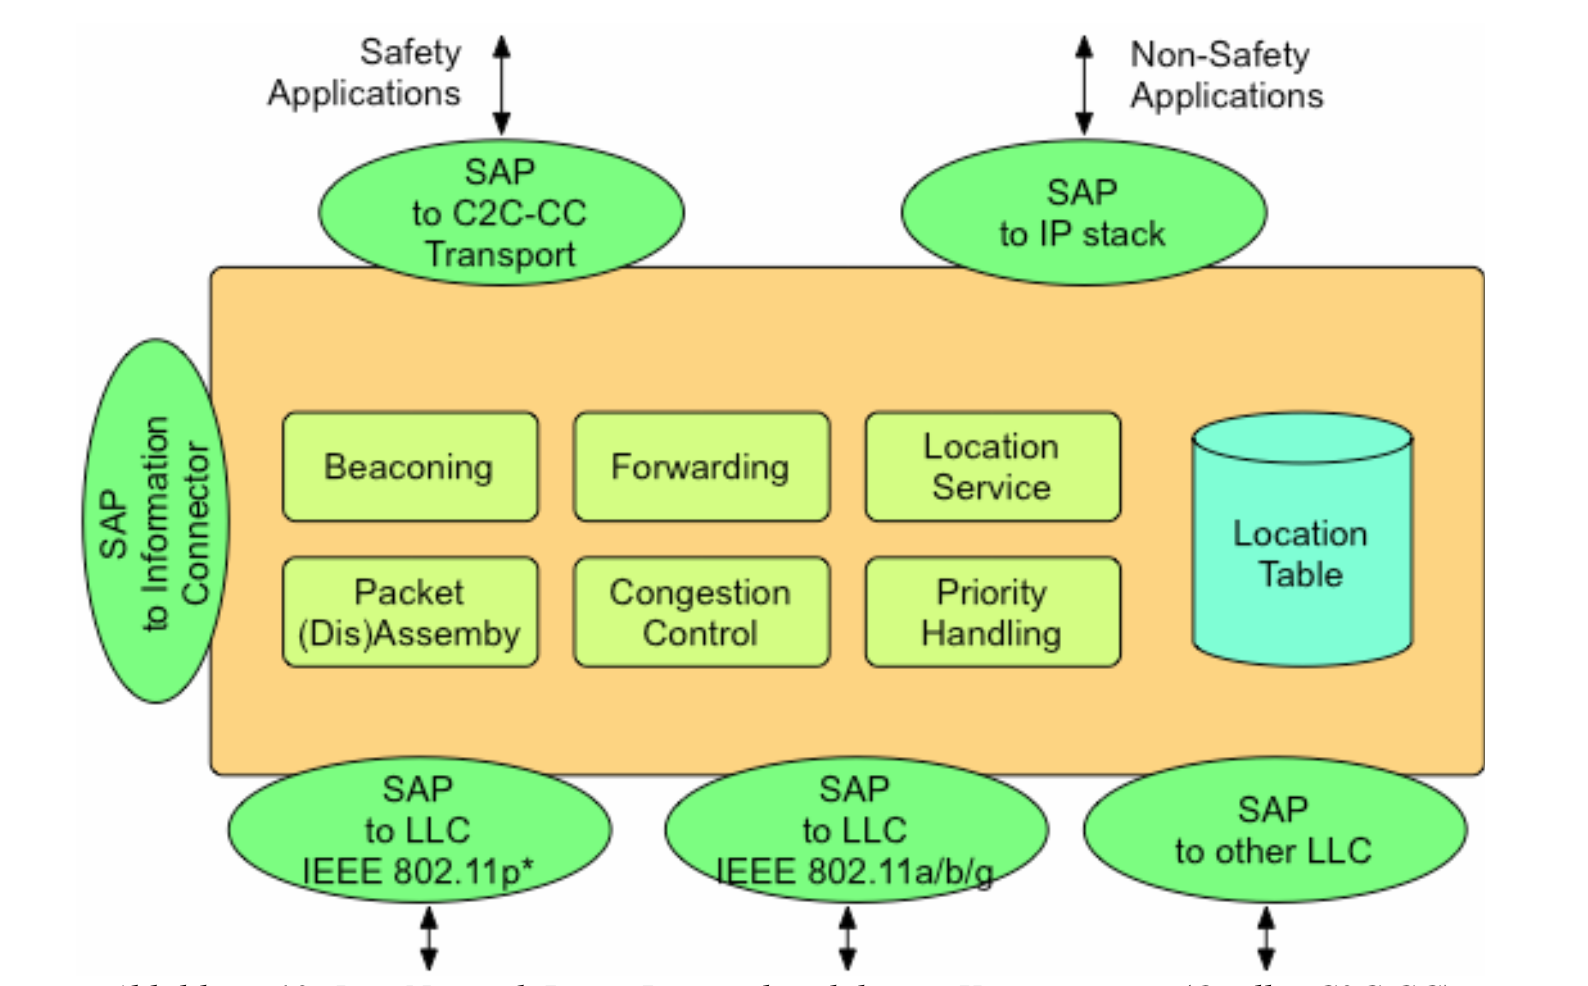
\includegraphics[width=0.99\textwidth]{content/images/03_networklayer/networklayer.jpg}
\caption{Die Komponenten des Networklayers}
\label{fig:nwl}
\end{figure}
Wie auf \autoref{fig:nwl} zu sehen befindet sich der Networklayer zwischen dem Aplicationlayer und dem Logical Link Control oder MAC-Layer. Das Protokoll das auf dem MAC-Layer läuft ist das, in der WLAN-Technik häufig genutzte CSMA/CA, das als bekannt vorausgesetzt wird. Es wird verwendet da sich mehrere Kommunikationseinheiten das selbe Medium teilen und es daher zu Kollisionen kommen kann. 

\subsubsection{Location Table}
\todo{neighbor tabelle hier mit einbeziehen etsi 7.1 da steht was da alles drin ist}
Jedes Fahrzeug verfügt über einen Location Table. In dieser Tabelle werden Informationen über die naheliegenden Knoten, also andere Fahrzeuge die C2C unterstützen, gespeichert. Diese Tabelle ist für das Forwarding notwendig da hier unter anderem die Adressen und Positionen der zu erreichenden Fahrzeuge gespeichert sind. 
Im Folgenden werden einige der Informationen aufgeführt die in einer solchen Tabelle enthalten sind. Jedoch können noch weitere Informationen dort gespeichert werden. Das genaue Format der Datensätze ist nicht spezifiziert und kann somit von diesem Dokument abweichen. Die Daten die in dem Location Table gespeichert sind sind nur zeitweise korrekt, daher sind sie mit einem Timestamp versehen und werden nach einer gewissen zeit verworfen. Die Informationen des Positionsvektors sollten mindestens über die unten aufgeführten Informationen verfügen. 
\begin{enumerate}
      \item C2C Netzwerkadresse
      \item MAC Adresse
      \item IPv6 Adresse
      \item Positionsvektor
      \begin{itemize}
      	\item Geschwindigkeit
	\item Heading
	\item Geo. Position
	\item Zeitstempel des Vektors
	\item Genauigkeit des Vektors
      \end{itemize}
      \item Version des Protokolls
      \item Typ des Fahrzeuges
      \item Zeitstempel des zuletzt erhaltenen Paketes
      \item Datenrate des ITS
      \item Direkter Nachbar Flag
\end{enumerate}

\subsubsection{Beaconing}
Um die Informationen in der Location Table zu füllen sendet jedes Fahrzeug im periodischen Abstand eine sogenannten Beacon-Nachricht an seine Umgebung. In dieser Nachricht sind die oben aufgeführten Informationen enthalten. Dadurch wird die Location Table von dem empfangenden Fahrzeug aktualisiert.

\subsubsection{Forwarding}
Der Networklayer untersützt verschiedene Arten von Forwarding Algorithmen diese werden im späteren Kapitel \autoref{sec:georouting} genauer erläutert.

\subsubsection{Location Service}
Da es durchaus vorkommen kann das der Location Table leer ist aber dennoch eine Nachricht gesendet werden muss, d.h. es wird nach einer Weiterleitungsmöglichkeit gesucht, existiert der Location Service. Über diese kann explizit nach Informationen eines Knoten gefragt werden der die Nachricht weiterleiten kann. Im vergleich zu den Beacon-Nachrichten ist der Location Service eher ein On-Demand Dienst der für Routenaufbau zuständig ist.
\begin{figure}
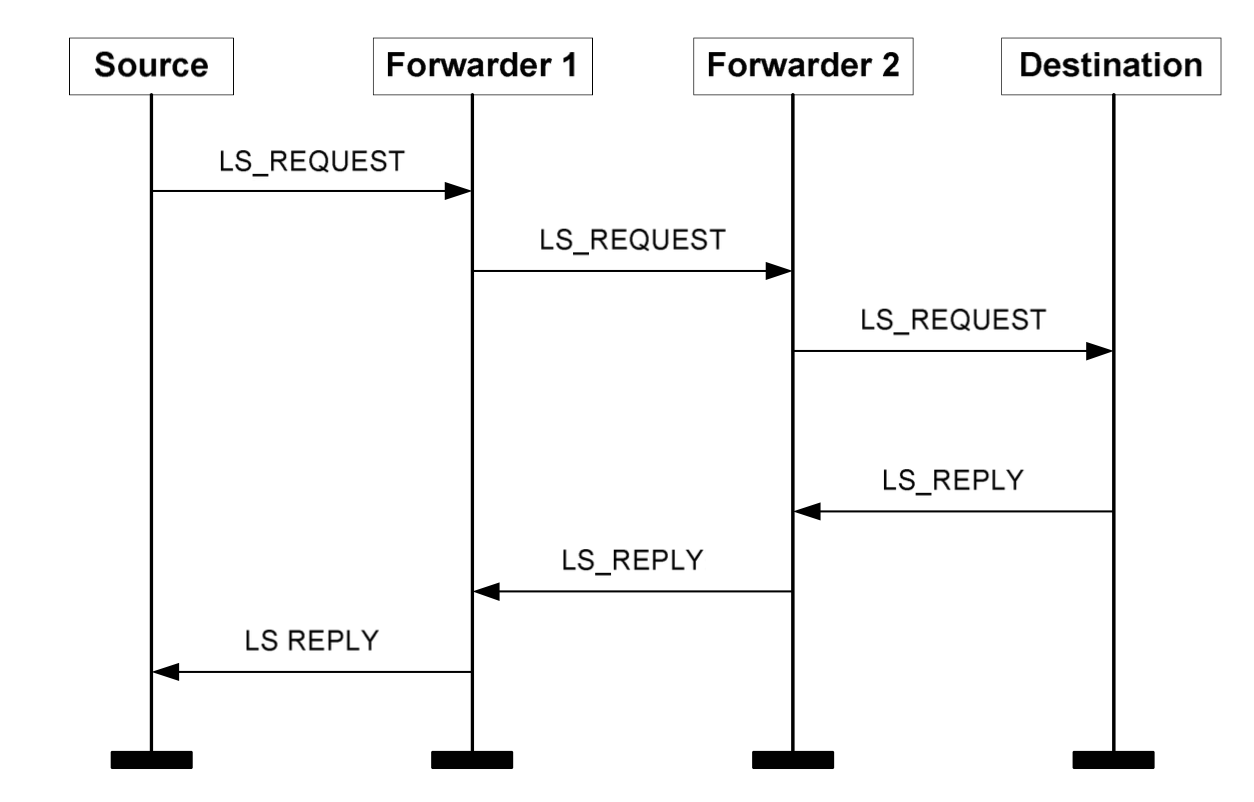
\includegraphics[width=0.99\textwidth]{content/images/03_networklayer/location-service-diagramm.jpg}
\caption{Ablauf einer Anfrage des Location Service}
\label{fig:locser}
\end{figure}
In \autoref{fig:locser} ist erkennbar wie über den Location Service Informationen des Ziels über zwei Forwarding Knoten abgerufen wird. 

\subsubsection{Priority Handling}
Anhand der Paketpriorität wird entschieden wie mit dem Paket verfahren wird. Damit wichtige Pakete zuerst gesendet werden können und andere dennoch empfangen werden gibt es eine Paketqueue in die die unwichtigeren Nachrichten eingereiht werden. 

\subsubsection{Packet Assemby}
Da sich beim versenden von Paketen die eigenen Positionsangaben sowie die Hops oder Time-to-Live ändern, muss der Networklayer dafür sorgen das die Pakete beim weitersenden modifiziert oder aktualisiert werden. Hierfür werden die Informationen aus der Location Table verwendet bevor das Paket weiter gesendet wird.

\subsubsection{Congestion Control}
Da die Paketdichte in einem C2C-Netz sehr hoch werden kann und es zu Überläufen oder Paketstaus kommen kann, muss in extremen Situationen das Netz reguliert werden. Hierauf wird in \autoref{sec:congestioncontrol} genauer eingegangen.

\section{Congestion Control\label{sec:congestioncontrol}}
\todo{Hier nochmal nachhacken ob es tatsächlich keine lösung gibt}
Noch ungeklärt sind die Transport- und Überlastungskontrolle. Offen sind Fragen bzgl. fehlerfreiem Transport (single protocol/multiple protocols), Prioritäten von Datenpacketen, Datenaggregation und Payloadgröße. Ausfallsicherheit (connection-free/conncetion-less), Forwarding (end-to-end Prinzip), Transportarten (unicast/broadcast), Fairness, Komplexität, Multiplexing sowie Verzögerungen und Ortsgültigkeit sind auch zu klären.Es bleibt abzuwarten, wie mit den Problemen umgegangen wird. Auf Grund der vielen Anforderungen muss höchste Sorgfalt in die Entwicklung gelegt werden. Eine Herausforderung ist z.B. die Frage der Ortsgültigkeit. Unter Ortsgültigkeit ist zu verstehen, wie lange eine Nachricht in einer bestimmten Region bei der sich schnell ändernden Netzwerktopologie gültig bleibt, oder als veraltet verworfen wird.

\section{Geo Routing\label{sec:georouting}}
Um in der \acl{C2C} die richtigen Routen zu finden und die Ziele zu adressieren benötigt jeder Teilnehmer in dem Netzwerk eine einmalige Adresse. Diese ist als \acl{GNW} Adresse spezifiziert. 

\subsection{Adressierung} 
Die \acl{GNW} Adresse besteht aus acht Bytes die verschiedene Informationen repräsentieren. Die ersten zwei Bytes zeigen ob die Adresse manuell oder Automatisch konfiguriert wurde, um was es sich für ein Fahrzeug handelt und den ITS-S Country Code. Die restlichen sechs Bytes repräsentieren die MAC Adresse.

\subsubsection{Konfiguration der Adressen}
\todo{siehe etsi Kapitel 9.2.1 duplicate address detection ist auch interessant}

\subsubsection{Duplicate address detection}
Um zu gewährleisten das die \acl{GNW} Adresse tatsächlich einzigartig ist, kommt die Duplicate address detection zum Einsatz. Sobald ein Empfänger eine Nachricht erhält. Vergleicht er seine eigene \acl{GNW} Adresse mit der des Paketes und danach die beiden MAC Adressen. Bei Übereinstimmung fordert er eine neue MAC-Adresse an. Und teilt dem System mit das eine Doppelte Adresse vorgefunden wurde. 

\subsection{Geo Unicast}
Um einen einzelnen Knoten zu Adressieren wird der Geo Unicast spezifiziert. Die Autos die zwischen Sender und der Empfangseinheit liegen dienen als Zwischenstationen. Über den Geo Unicast werden Nachrichten entweder über einen Hop an das Ziel gesendet oder über Zwischenstationen mit mehreren Hops. Die Nachricht kann bei den Zwischenstationen verändert werden. Das heisst zwei oder mehr Nachrichten werden zu einer zusammengefasst bevor sie weitergesendet werden. Dieser Vorgang ist auch umgekehrt durchführbar, sodass eine Nachricht aufgeteilt werden kann. Der Inhalt der Nachricht kann ebenfalls verändert oder Informationen hinzugefügt werden. 

\begin{figure}
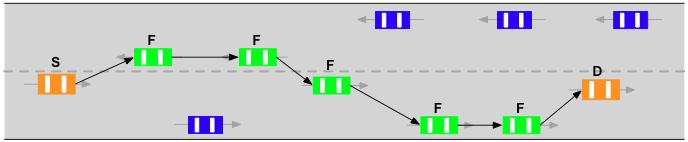
\includegraphics[width=0.99\textwidth]{content/images/03_networklayer/GeoUnicast.jpg}
\caption{Geo Unicast \cite{etsi102636-1}}
\label{fig:geounicast}
\end{figure}

\subsection{Topologically-scoped broadcast}
Der Topologically-scoped broadcast sendet einen Nachricht mit einem bestimmten Hop Count an alle um den Knoten erreichbaren Einheiten. Diese Nachricht wird dann von den Knoten empfangen, bei denen der Hop Count endet.

\begin{figure}
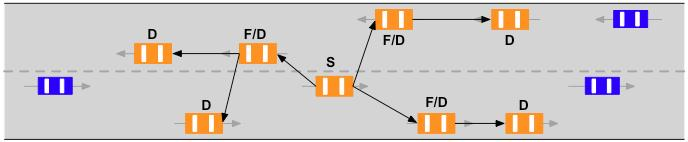
\includegraphics[width=0.99\textwidth]{content/images/03_networklayer/TSC.jpg}
\caption{Topologically-scoped broadcast mit Hop Count 2 \cite{etsi102636-1}}
\label{fig:tsc}
\end{figure}


\subsection{Geographically-scoped broadcast}
Über den Geographically-scoped broadcast ist es einem Knoten möglich, um sich herum oder in einer bestimmten Entfernung zu sich selbst eine definierte Region zu erreichen. 

\begin{figure}
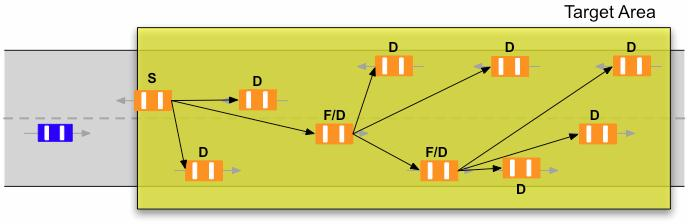
\includegraphics[width=0.99\textwidth]{content/images/03_networklayer/GSB.jpg}
\caption{geographically-scoped broadcast \cite{etsi102636-1}}
\label{fig:gsb}
\end{figure}
